% XeTeX-Header zur Definition des Dokuments
% XeTeX-Vorlage für Abschlußarbeiten an der Universität Bielefeld
% ---------------------------------------------------------------------
% Stand, 07. Juni 2010
%
% Timo Reuter (treuter@cit-ec.uni-bielefeld.de), AG Semantic Computing
% Exzellenzcluster für Cognitive Interaction Technology
%
% Dies Vorlage setzt die Schriftart FagoNo sowie einen XeTeX-Kompiler 
% voraus. Alle Dokumente müssen zwingend mit Unicode (UTF-8) als
% Kodierung abgespeichert werden.

\documentclass[
  a4paper,              % Wir verwenden A4 Papier
  %oneside,             % Einseitiger Druck
  twoside,              % Zweiseitiger Druck
  12pt,                 % Große Schrift, besser geeignet für A4
  halfparskip,          % Halbe Zeile Abstand zwischen Absätzen
  chapterprefix,        % Kapitel mit 'Kapitel' anschreiben
  headsepline,          % Linie nach Kopfzeile
  footsepline,          % Linie vor Fußzeile
  bibtotocnumbered,     % Literaturverzeichnis im Inhaltsverzeichnis numeriert einfügen
  DIV=15,
  BCOR=8mm
]{scrbook}

% Kopf-/ und Fußzeilen
\usepackage{footmisc}

% Parts haben im Inhaltsverzeichnis keine Seitenzahlen
\makeatletter
\let\partbackup\l@part
\renewcommand*\l@part[2]{\partbackup{#1}{}}
\makeatother

% Zeichencodierung des Dokuments und des Zeichensatzes.
\usepackage{pifont}
\usepackage{fontspec}
\usepackage{xunicode}
\usepackage{xltxtra}
\usepackage{textcomp}
\usepackage{csquotes}

% Lokalisierung auf deutsch (Silbentrennung usw.)
%\usepackage[german]{babel}
\usepackage[english]{babel}

% Paket um Grafiken im Dokument einbetten zu können.
\usepackage{graphicx}
\graphicspath{{images/}}

% PDF-Merkmale
\usepackage[
  pdftitle={Memory-based exploratory online learning of simple object manipulation},            % Titel des PDF Dokuments.
  pdfauthor={Jan Pöppel},                 % Autor des PDF Dokuments.
  pdfsubject={Memory-based exploratory online learning of simple object manipulation},          % Thema des PDF Dokuments.
  pdfcreator={Texlive, XeTeX},           % Erzeuger des PDF Dokuments.
  pdfkeywords={Keyword1, keyword2},      % Schlüsselwörter für das PDF.
  pdfpagemode=UseOutlines,               % Inhaltsverzeichnis anzeigen beim Öffnen
  bookmarksopen=false,                   % Inhaltsverzeichnisbaum geöffnet anzeigen
  pdfdisplaydoctitle=true,               % Dokumenttitel statt Dateiname anzeigen.
  pdflang=en                             % Sprache des Dokuments.
]{hyperref}

% Schriften
\defaultfontfeatures{Mapping=tex-text}
\setmainfont[ItalicFont={FagoNo}, BoldFont={FagoNoLf-Bold}]{Latin Modern Roman} %{GoudyOlSt BT}
\setsansfont{FagoNo}
%{\setmonofont{Arial}\fontsize{48pt}{\baselineskip}\selectfont}
%\usepackage{default}

% Farben definieren
\usepackage{color, colortbl}
\definecolor{LinkColor}{rgb}{0,0,0}
\definecolor{ListingBackground}{rgb}{0.85,0.85,0.85}
\definecolor{LightGrey}{rgb}{0.93,0.93,0.93}
\definecolor{LightGrey2}{rgb}{0.9,0.9,0.9}
\definecolor{DarkGrey}{rgb}{0.65,0.65,0.65}
\definecolor{UniBiGreen}{rgb}{0.0,0.457,0.336}
\definecolor{CitecOrange}{rgb}{0.93,0.453,0.004}

% Farbeinstellungen für die Verweise im PDF-Dokument.
\hypersetup{
  colorlinks=true,       % Aktivieren von farbigen Verweisen im Dokument (ohne Rahmen)
  linkcolor=LinkColor,   % Farbe festlegen.
  citecolor=LinkColor,   % Farbe festlegen.
  filecolor=LinkColor,   % Farbe festlegen.
  menucolor=LinkColor,   % Farbe festlegen.
  urlcolor=LinkColor,    % Farbe von URL's im Dokument.
  bookmarksnumbered=true % Überschriftsnummerierung im PDF Inhalt anzeigen.
}

% Beschriftungen für Bilder und Tabellen
\setcapindent{1em} % Zeilenumbruch bei Bildbeschreibungen.
\setkomafont{captionlabel}{\fontspec[Color=656565, Scale=0.7]{FagoNoLf-Bold}} % Beschriftungen für Bilder und Tabellen
\setkomafont{caption}{\fontspec[Color=656565, Scale=0.7]{FagoNoLf-Bold}} % Beschriftungen für Bilder und Tabellen
\setkomafont{descriptionlabel}{\fontspec{FagoNoLf-Bold}} % Optionales Label in der description-Umgebung


% Stil der Kopf- und Fußzeilen
\usepackage[footsepline,plainfootsepline]{scrpage2}
\pagestyle{scrheadings}
\setheadsepline{}[\color{DarkGrey}]    % Kopfzeilenlinie
\setfootsepline{}[\color{DarkGrey}]    % Fußzeilenlinie
\renewcommand*{\partpagestyle}{empty}  % Parts haben keine Kopf-/Fußzeile

% Überschriften
\setkomafont{sectioning}{\normalfont\bfseries} % Titel mit Normalschrift
\addtokomafont{sectioning}{\fontspec{FagoNoLf-Bold}}
\addtokomafont{pagehead}{\fontspec[Color=656565]{FagoNoLf-Bold}}   % Seitentitel
\addtokomafont{pagenumber}{\fontspec[Color=656565]{FagoNoLf-Bold}} % Fußnoten

% Stil der Überschriften
\usepackage[Lenny]{sty/fncychapleo}

% Paket um Quelltext sauber zu formatieren.
%\usepackage[savemem]{listings}
%% Einstellungen für das 'listings' Paket.
%\lstloadlanguages{C}            % Sprache laden, notwendig wegen Option 'savemem'
%\lstset{
%	language=C,                 % Sprache des Quelltexts ist C
%	numbers=left,               % Zelennummern links
%	stepnumber=1,               % Jede Zeile numerieren.
%	numbersep=5pt,              % 5pt Abstand zum Quellcode
%	numberstyle=\tiny,          % Zeichengröße 'tiny' für die Nummern.
%	breaklines=true,            % Zeilen umbrechen, wenn notwendig.
%	breakautoindent=true,       % Nach dem Zeilenumbruch Zeile einrücken.
%	postbreak=\space,           % Bei Leerzeichen umbrechen.
%	tabsize=2,                  % Tabulatorgröße (Indent) ist 2
%	basicstyle=\ttfamily\scriptsize, % Schrift
%	showspaces=false,           % Leerzeichen nicht anzeigen.
%	showstringspaces=false,     % Leerzeichen auch in Zeichenketten ('') nicht anzeigen.
%	extendedchars=true,         % Alle Zeichen vom Latin1 Zeichensatz anzeigen.
%	backgroundcolor=\color{ListingBackground}, % Hintergrundfarbe des Quelltexts setzen.
%	captionpos=b,               % Caption unten
%    %linewidth=0.9\textwidth,   % base line width
%    xleftmargin=0.02\textwidth, % margin left
%    xrightmargin=0.02\textwidth % margin right
%}


\usepackage[linesnumbered]{algorithm2e}
\SetAlFnt{\ttfamily\small}

\usepackage{amsmath}
%\DeclareMathOperator*{\argmin}{arg\,min}
\newcommand{\argmin}{\operatornamewithlimits{argmin}}

\usepackage[e]{esvect}
\makeatletter
\def\traitfill@#1#2#3#4{%
  $\m@th\mkern2mu\relax#4#1\mkern-6.0mu%
   \cleaders\hbox{$#4\mkern0mu#2\mkern0mu$}\hfill%
   \mkern-1.5mu#3$%
}
 \makeatother
\renewcommand{\vec}[1]{\vv{#1}}

% Tabellen
\usepackage{array}                  % Paket für erweiterte Tabelleneigenschaften
\usepackage{multirow}               % Zusammengefaßte Reihen in Tabellen ermöglichen
\setlength{\arrayrulewidth}{0.7pt}
\setlength{\extrarowheight}{3pt}
\arrayrulecolor{DarkGrey}           
\usepackage{longtable}              % Ermöglicht sich über mehrere Seiten erstreckende Tabellen
\usepackage{tabularx}               % Mächtigere Tabellenumgebung


% Stil für Designboxen
\newcommand{\designbox}[2]{
  \hspace*{17pt}
  \begin{tabular*}{402pt}{p{378pt}p{0pt}}
    \begin{flushright}\fontspec[Color=656565, Scale=0.9]{FagoNoLf-Bold}#1\hspace*{-18.5pt}\vspace*{-16pt}\end{flushright}\\
    \hline
    \cellcolor{LightGrey}\fontspec{FagoNo}#2 & \cellcolor{DarkGrey}\\
    \begin{picture}(0,0)
      \put(245,13){\color{DarkGrey}\rule{151pt}{0.5pt}}
    \end{picture}
  \end{tabular*}
}

% Bibliographie-Stil
%\usepackage{apacite}         % Psychologie
\usepackage[numbers]{natbib}  % Linguistik und Naturwissenschaften

% Silbentrennung für Wörter, die nicht vom Babel-Paket erkannt werden
\hyphenation{Dezi-mal-trenn-zeichen In-stal-la-ti-ons-as-sis-tent}

%Abkürzungen
%\usepackage{acronym}

%Glossary and Acronyms

\usepackage[nomain,toc,acronyms]{glossaries}
%\chapter{Acronyms}
%\begin{acronym}[Bash]
% \acro{ITM}{Instantaneous Topological Map}
% \acro{GNG}{Growing Neural Gas}
% \acro{LLM}{Local Linear Map}
%\end{acronym}

\newacronym{itm}{ITM}{Instantaneous Topological Map}
\newacronym{aitm}{AITM}{Adapted Instantaneous Topological Map}
\newacronym{gng}{GNG}{Growing Neural Gas}
\newacronym{llm}{LLM}{Local Linear Map}
\newacronym{nn}{NN}{Nearest Neighbour}
\newacronym{knn}{\textit{k}-NN}{k-Nearest Neighbour}
\newacronym{rnn}{RNN}{recurrent neural network}
\newacronym{bn}{BN}{Bayesian Network}
\makeglossaries
% Überschriften anpassen
%\usepackage{titlesec}
%\titleformat{\subsection}{\bfseries\large\sffamily\itshape}{}{0em}{\thesubsection~}
% Folgende Dinge tut man in TeX NICHT, da das Ganze gegen die Grundregeln des
% Textsatzes verstößt. Wer meint, es trotzdem verwenden zu müssen, um ein "Word"-ähnlicheres 
% Satzbild zu bekommen, sollte mit dem Verantwortlichen über Sinn oder Unsinn dieses 
% Vorhabens diskutieren und diese "Hacks" möglichst unterlassen.

% Zeilenabstand ändern (Standard bei TeX ist 1,2)
%\usepackage{setspace}
%\onehalfspacing % Ergibt 1,5 Zeilenabstand
%\doublespacing % Ergibt 2,0 Zeilenabstand

% Seitenränder ändern
%\usepackage{anysize}
%\marginsize{2.5cm}{2cm}{2.5cm}{2.5cm}




\begin{document}
  % Römische Nummerierung für Einleitung mit Index usw.
  \pagenumbering{roman}

  % Titelseite definieren
\begin{titlepage}

  % Alles zentriert darstellen
  \begin{center}

    \setlength{\unitlength}{1mm}
    
    % Graphische Elemente auf der Seite platzieren
    \begin{picture}(0,0)
      \put(-55,5){\color{CitecOrange}\rule{15cm}{5mm}}
      \put(-105,-10){\color{CitecOrange}\rule{20cm}{1.52cm}}
      \put(-105,-15){\color{CitecOrange}\rule{18cm}{5.2mm}}
      
      \put(-40,-8){\fontspec[Color=fefefe, Scale=3.6]{FagoNoLf-Bold}Master Thesis}

      %\put(-90,12){\color{UniBiGreen}\rule{12mm}{12mm}}
     % \put(-84,10){\color{UniBiGreen}\rule{29mm}{10mm}}      
     % \put(-82.5,12){\fontspec[Color=fefefe, Scale=0.66]{FagoNoLf-Bold}Universität Bielefeld}
      
      \put(-90,-230){\color{CitecOrange}\rule{20cm}{2.5mm}}
    \end{picture}

    \vspace{3cm} % Vertikaler Abstand von 25pt

    % Name der Universität, der Fakultät und (optional) des Studiengangs
    {\fontspec[Color=101010, Scale=2.0]{FagoNoLf-Bold}Bielefeld University} \\
    \vspace{10pt} % Vertikaler Abstand von 10pt
    {\fontspec[Color=101010, Scale=1.7]{FagoNo}Faculty of Technology }
    %\vspace{10pt} % Vertikaler Abstand von 10pt
    %{\huge Studiengang ISY}

    \vspace{35pt} % Vertikaler Abstand von 35pt

    % Titel der Arbeit
    {\fontspec[Color=101010, Scale=2.5]{FagoNoLf-Bold} Memory-based exploratory online learning of simple object manipulation} \\
    \vspace{10pt} % Vertikaler Abstand von 10pt
    %{\fontspec[Color=101010, Scale=2.5]{FagoNoLf-Bold} \textbf{einen schönen Titel hat}} \\
    %\vspace{10pt} % Vertikaler Abstand von 10pt

    \vspace{40pt} % Vertikaler Abstand von 40pt

    % Angestrebter Abschluß wird hier eingetragen (B.Sc./M.Sc./B.A./etc.)
    {\fontspec[Color=101010, Scale=1.0]{FagoNo}In Partial Fulfillment of the Requirements for the Degree of} \\
    \vspace{5pt}
    {\fontspec[Color=101010, Scale=1.5]{FagoNoLf-Bold}Master of Science (M.Sc.)}

    \vspace{40pt} % Vertikaler Abstand von 40pt

    % Name des Students/der Studenten
    {\fontspec[Color=101010, Scale=1.5]{FagoNo}Jan Pöppel} \\
    \vspace{5pt} % Vertikaler Abstand von 5pt
  
    % Monat und Jahr der Arbeit (Abgabedatum)
    {\fontspec[Color=101010, Scale=1.2]{FagoNo}September 2015}

    \vspace{50pt} % Vertikaler Abstand von 40pt

  \end{center}

    {
      \begin{tabular}{ll}
        \vspace{5pt} % Vertikaler Abstand von 5pt
        \fontspec[Color=101010, Scale=1.0]{FagoNo}Referee:  & \fontspec[Color=101010, Scale=1.0]{FagoNo}Apl. Prof. Dr.-Ing. Stefan Kopp \\
        \vspace{5pt} % Vertikaler Abstand von 5pt
        \fontspec[Color=101010, Scale=1.0]{FagoNo}Referee: & \fontspec[Color=101010, Scale=1.0]{FagoNo}Dipl.-Inf. Maximilian Panzner \\
      \end{tabular}
    }
    


\end{titlepage}
  % Abstract

% Der Abstract wird nicht ins Inhaltsverzeichnis aufgenommen

%\chapter*{\enskip Abstract}

%Dies ist eine gute Zusammenfassung, warum der Leser diesen Text lesen sollte.

% Übersetzte Version
\chapter*{\enskip Abstract}

The classical machine learning approach is to train suitable models on reasonable big data sets before deployment. However, this approach is not suitable in many scenarios such as robotics due to scarcity of data. Furthermore, general purpose robots are expected to be able to deal with unknown circumstances. This requires the ability to incrementally adapt to unknown situations.

This thesis considers learning about simply object manipulations such as pushing as a simplified scenario of adapting to unknown environments.
Within this context, this thesis suggests and discusses two memory-based concepts that challenge the tasks of incremental online learning with limited domain knowledge.
The concepts learn forward and inverse models of their environment, allowing them to predict future states as well as incrementally reach desired target states.

The learned forward and inverse models of the environment's dynamics are evaluated separately in different scenarios.
The evaluations show that the proposed methods both successfully learn to predict future states and interact with their given environment while providing insight of remaining problems.


 % Abstract
  %% Widmung/Zitat/Motto der Arbeit

\cleardoublepage

  ~
  \vspace{370pt} % Vertikaler Abstand von 370pt

  \begin{tabularx}{0.9\textwidth}{Xl}
      & {\large »Hier könnte eine} \\
      & {\large Widmung für jemanden} \\
      & {\large stehen«} \\
  \end{tabularx}

  \vspace{0pt}

  \begin{tabularx}{0.9\textwidth}{Xr}
      & \textit{Zitierter Autor}\\
  \end{tabularx}

\cleardoublepage
 % Widmung/Zitat
  
  \tableofcontents  % Inhaltsverzeichnis
  %\listoffigures    % Bildverzeichnis
  %\listoftables     % Tabellenverzeichnis

  \cleardoublepage  % Seitennummerierung neustarten

  % Arabische Nummerierung für den Hauptteil
  \pagenumbering{arabic}
  
  % Einzelne Kapitel werden hier eingefügt
  \chapter{Introduction}

%Motivate necessity
%State goals
%Structure of thesis
%What is the problem that we try to solve?
%Why is it relevant to solve it?


%TODO delete? Most likely not good...
%The defining quality that any agent, artificial or natural, requires is learning. Also used for many different 
%phenomenons, the term learning at its core means adaptation. The agent or some part of it adapts in order to
%better deal with its environment. Natural agents, especially humans, display impressive learning capabilities,
%allowing them to quickly adapt to ever changing environments and new tasks.
%
%In recent years, machine learning has come a long way in understanding and reproducing some of the learning
%capabilities of humans. We now have a wide range of different techniques and algorithms that can yield good
%classification and regression results. %TODO make glossary to explain what classification and regression is
%In introduction to these can for example be found in book by Bishop \cite{bishop}.
%
%The quality of the results achieved by machine learning is however more dependent on the chosen representation
%of the problem then on the actual technique used. For example it is generally not sufficient to use the raw audio signals 
%for speech recognition \cite{speechRecog}. Instead most speech recognizers use carefully selected pre-computed
%features that allow the underlying machine learner to correctly distinguish the words. 
%
%Because finding the best features is as challenging as learning a problem itself, a lot of focus as recently 
%shifted to deep learning \cite{deepLearning}. Deep learning is a technique that is inspired by the human brain and refers to
%training neural networks with many thousands of artificial neurons. Properly trained, these networks are capable of finding 
%relevant features in the presented data by themselves \cite{deepLearningFeatures}. Currently the biggest
%problem with deep learning is the required amount of training before the network can be used successfully. Although recent
%advances such as the development of Hinton's dropout technique \cite{dropout} allows to train bigger networks with fewer data,
%this criteria still limits the potential use cases of deep learning and neural networks in general.

After decades of research a vast amount of powerful tools have been developed for machine learning. A good overview can be found in the book by Bishop \cite{bishop}. Each of these methods has its own advantages and disadvantages and are applicable to certain situations. Currently, research in machine learning is often performed by choosing a problem, e.g. image recognition or movement control, and trying to find and tune the most successful method to solve the chosen problem. This way the researchers were able to create better classifiers for image recognition (e.g. \cite{imageRecList}) and better controllers for complex movements (e.g.\cite{movementList}).
%TODO Adrianas Anmerkung: 1. Im ersten Absatz würde ich das "e.g. image recognition or movement
%control" weglassen. Das kommt direkt im nächsten Satz schon wieder
%(und image recognition im 3. Absatz noch einmal), das stört dann etwas
%den Lesefluss, wenn man so denkt "häh, déjà vu?!"


In most of these cases the machine is trained to solve one specific problem. Depending on the chosen methods it is not possible to extend the machines knowledge easily without retraining the entire system afterwards because of the stability-plasticity-problem \cite{stability-plasticity}. More precisely because of the phenomenon of catastrophic forgetting \cite{catastrophicForgetting1}.

With advances in robotic hardware and the successful application of machine learning in specialized tasks, such as image recognition, the goal of robotic research trends towards multi-purpose robots. However, the biggest problem for multi-purpose machines is that the current approach to machine learning is not applicable. Since the number of tasks the robot has to face is not known in advance, suitable tools cannot be training in advance. Furthermore, even if one would attempt to train specialized parts for all kinds of problems, acquiring sufficient and accurate training data beforehand is infeasible at best. 
%TODO glossary for model or some footnode on what is meant by model
Therefore, instead of trying to train the machine beforehand, it might be better to provide it with the means to adapt to new situations on its own while it is encountering them. Instead of learning on previously recorded training data, the robot adapts its model to the continuous stream of data while it is already using what it learned beforehand. The biggest reason against such an continuous incremental approach is its difficulty. When incrementally training a single model to solve multiple different problems, the catastrophic forgetting effect is usually experienced. The usual approach is learn local models for each task separately, however this introduces the need to recognize and distinguish the different problems in order to know which kind of local model the robot needs to employ. 

Instead of challenging the entire problem of incrementally learning an unlimited number of arbitrary tasks, this thesis concentrates on the incremental learning of one task without prior training. 
While there are multiple machine learning methods that allow incremental updates, not all of them are suitable for this kind of task. First of all, the method should be as independent on prior knowledge as possible so that it can be used for a wide variety of task the robot might encounter. Furthermore, the update and query times of the chosen method need to be quick enough to allow continuous interaction with the environment. On top of that, the chosen method should not suffer from the catastrophic forgetting effect since the robot would constantly keep updating it. For this thesis a memory based learning approach was chosen in order to solve these problems. Due to their one-shot learning ability, memory based methods can produce good prediction results from very little training data. 

One important aspect of general purpose robotics is object manipulation. In order to successfully interact with the objects in its environment the robot needs to learn what kind of interactions are possible and what their effects are. 
Furthermore, object interactions are hard to model manually as they follow complex dynamics. On top of that, different object can behave completely differently, so that knowledge acquired in previous training sessions might not be useful later on. It is for these reasons object interactions make an ideal target for online self adaptation. 

This thesis provides two concepts that provide incremental learning of pushing interactions between an actuator controlled by action primitives and some object in the environment.
While pushing interactions are only a very small subset of possible interactions a robot can have with objects, their dynamics still provide sufficient complexity to evaluate incremental learning systems. Since the behavior of differently shaped objects can vary a lot, learning about different kind of objects can even be regarded as learning similar but different tasks.%TODO Maybe more on this?
The proposed concepts need to provide a forward model as well as an inverse model. The forward model makes predictions about the state of all entities in the environment after an action primitives as been performed. The inverse model provides an action primitive that is used to reach a specified target configuration within the environment.

The goal of this thesis can summarized to provide and evaluate simple models that:
%TODO planning and lifelong are mentioned here for the first time and not explained!!!
\begin{enumerate}
	\item Update themselves incrementally during the interaction
	\item Allow prediction and planning of simple object interactions % with minimal domain knowledge
	\item Allow lifelong learning
\end{enumerate}

This thesis is structured as follows: In chapter \ref{chap:stateOfTheArt} an overview over memory based learning as well as recently proposed models for learning object interactions for robotics is given. Two concepts were developed in order to fulfill the stated goals. Their general idea is described in \ref{chap:concept} before concrete implementation details are given in chapter \ref{chap:modelReal}. These models are then evaluated with regards to their prediction and planning performance in chapter \ref{chap:evaluation}. Finally, this thesis concludes with a discussion of these results in chapter \ref{chap:conclusion}.


  \chapter{State of the art}



  \chapter{Concept}

In order to achieve the desired results, multiple models were 
developed incrementally. This chapter explains the different 
concepts in general. Details on the concrete realizations of these models can 
be found in chapter \ref{chap:modelReal} while their evaluation and discussion 
can be found in chapters \ref{chap:evaluation} and \ref{chap:conclusion} 
respectively. %TODO consider removing if it is written at the end of the 
%introduction
The first concept, explained in section \ref{sec:pairInteractions}, uses a 
pairwise interaction representation. In contrast to that, section 
\ref{sec:objectChange} describes the second concept, which represents the 
individual objects and models the change in their dynamics.

\section{Memory based models\label{sec:mbm}}
%TODO do I need such a section and if, should it be here?
TODO? Vl besser bei technologies?

The general idea of memory based learning, also called instance based learning, is to use lazy 
generalization. This means that the system compares a new problem instance with previously seen 
training examples in order to make a prediction instead of using an explicit generalization that 
was computed during training. 

The simplest memory based approach is to simply store the training data as 
input-output pairs in memory. When querying the model, for example in order to 
make a prediction, a nearest neighbor search \cite{nearestNeighbor} is 
performed on the inputs for all seen training examples and the corresponding 
output of the most similar pair is return as the prediction.

The advantages of such an approach are that there is no catastrophic forgetting during online 
learning, since the model only changes locally around each newly inserted data 
point. Furthermore, the required amount of training data is very limited as 
long as it is very similar to the test situation. In fact, depending on the 
query task, a single trained input-output pair can be enough to provide a 
reasonable prediction. 

The disadvantages are increasing query times as the model grows since most of the work is performed then. On top of that, the simple model does not generalize well in between training points if there are big changes. (TODO show graph to visualize this) %TODO add image showing this?

Multiple approaches have been proposed in order to reduce the gravity of the 
disadvantages such as using index structures to increase nearest neighbor 
search or using different methods in order to smooth the model output, for 
example by interpolating between the closest k points. 
%Section \ref{sec:ITM} 
%goes into more details about the underlying memory based structure that was 
%used for this thesis. 
%TODO maybe remove this here, since ITM is not really the memory based model, 
%just part of it/the predictor -.-

A memory based approach was mainly chosen due to the good online training 
capabilities and the one shot learning properties for this thesis.

The different concepts presented here try to structure and cluster the training 
data in order to guide training and improve prediction.

\section{Pairwise interactions\label{sec:pairInteractions}}
%TODO remove/rename word episode or explain it properly!. The concept is 
%independent of the timeframe

The first developed model adopted the commonly used idea of modeling object 
interaction by concentrating on pairwise interactions, also used by 
\cite{pairwise interaction}. The idea is to not model each object for itself 
but rather model the interaction between them by using features that describe 
their relative attributes (see section \ref{sec:pairStates} for details about 
the chosen representation). 
When predicting the next object state, the next interaction state is predicted 
first and the resulting object states are extracted from there afterwards. The 
input for model consists of the current interaction features between two 
objects and the chosen action. The output represents the change from the input 
in the next state.

In order to reduce the query costs the model tries to cluster similar 
interactions in more abstract collections, that are called \enquote{abstract 
episode collections} here. The general idea is visualized in figure \ref{fig:pairIdea}.

\begin{figure}
%TODO make image
\caption{TODO Visualization of pairwise concept}
\label{fig:pairIdea}
\end{figure}


\subsection{Abstract episode collections}

In order to avoid the nearest neighbor search on all recorded episodes, this 
model tries to cluster the experiences it made into more abstract collections.
The clustering is performed based on the set of attributes that changed within 
each episode. The set $S$ of attributes that changed is defined as follows 
\begin{equation}
S = \{f | f \in F ~ \wedge ~ ||Pre(f)-Post(f)|| > \epsilon_{Noise}\}
\end{equation}
where $F$ denotes the set of all features, $Pre(f), Post(f)$, the value of 
feature $f$ in the initial and resulting state of the episode respectively and 
$\epsilon_{Noise}$ a threshold to cancel out small noise.

For each different set the model creates a new abstract collection $AC_i$. The 
idea is that these collections correspond to different interaction scenarios. 
The set $\{spos\}$ for example corresponds to the interaction of pushing the 
object directly in the center, since the distance and relative velocities do not 
change between the two objects. The set $\{dpos, dist\}$ on the other hand 
describes the interaction of the actuator moving without contact to the object. 
The abstract collection effectively split the interaction space in subregions. 

\subsection{Prediction}

Prediction is performed by following a winner-takes-all approach:
%the idea of mixture of experts 
%\cite{mixtureExperts}: 
When predicting, the model first estimates the collection that is most likely 
responsible for the next episode and uses the collection to make the 
prediction. 

By training a classifier, e.g. a decision tree \cite{DT}, on all the 
input-collection pairs, that were already seen, this selection becomes 
independent of the number of training examples already stored. The total number 
of collections is limited to the size of the superset of $F$, although in 
practice, not all possibilities are likely and only those collections are 
considered, that are already made up of more than $\epsilon_{min}$ training 
examples. 
This threshold is used to reduce the number of outliers when training the 
classifier.  

After the suitable collection has been selected, one could perform nearest 
neighbor search on the episodes of that collection in order to make the 
prediction. However, since the number of episodes can grow quite rapidly, each 
collection trains it's own local predictor. 
%TODO if you put something like this here, make sure you show results that %support something like 
%this: 
%By splitting the entire interaction space into 
%subregions, each local predictor can be much simpler than one model that tries 
%to predict the entire space.
This also allows the model to remove stored episodes when the local predictors 
are already trained sufficiently well. 

In order to reduce the burden on the manual feature and metric selection, an 
automatic feature selection can be performed periodically in each abstract 
collection in order to improve the performance of the local predictors. %TODO 
%show comparison in results

\subsection{Planning}
%TODO
(TODO consider redoing the planning algorithm more similar to the way it is done
in the most recent model, which works, maybe the same ideas can be employed 
here)

In order to get a suitable action given a target configuration, the model first computes the 
difference set between the current situation and the target 
configuration. The model then searches for an abstract episode collection that 
corresponds to the same set of attributes and delays the action computation to 
that collection. In case the model does not yet now of such an collection, the 
most similar collection is chosen instead, meaning the collection that covers 
most of the changed attributes in the computed difference set. 

The abstract collection queries it's own inverse model, which can be the same 
as their predictor, if that model supports bidirectional queries, for the 
action that produces the output most similar to the desired target. 

[TODO FORMEL] %TODO

The model can then use it's forward model in order to check if the selected 
action is applicable in the current situation and if it indeed reduces the 
distance to the target. In case no suitable action could be selected, the model 
can choose to perform a random action, in order to experience new interactions, 
that will improve the following predictions and planning results.


\subsection{Theoretical problems}

The biggest problem with the pairwise interaction based approach is that it 
does not model the interactions between multiple objects. In a scenario with 
two objects alongside the actuator, it is not trivial to decide which pairwise 
interaction should be used to predict the next state of each of the objects, 
even if only two entities interact. In interaction scenarios where all three 
objects are touching at least one of the other objects, the pairwise 
representation fails completely since it can only represent effects between two 
of them at any given time. 

\begin{itemize}
\item AC selection
\item Number of samples increases a lot (even without interaction/touch, the interaction states 
differ -> one AC gets trained)
\begin{itemize}
\item The most simple AC (no interaction, just actuator movement) becomes the slowest
\end{itemize}
\end{itemize}


\section{Object states and global changes\label{sec:objectChange}}
(TODO
Maybe actually drop this concept or briefly mention it as intermediate step to the current, best 
working model?)


In order to avoid the problem of multiple objects, a second concept was 
developed. Instead of pairwise interactions the objects are modeled 
individually by object states (see section \ref{sec:objectStates} for details about the used representation and features). 
Predictions are made solely based on \enquote{local} features for each object. 
Local means here, that an object predicts e.g. it's next position only based on it's
current features, such as position and velocity. 
In order to be able to predict the effects of interactions such as collisions, 
another layer of predictors is introduced that predict the \enquote{global} 
changes on the dynamics of each object. Here global means, that other objects 
are used to compute the used features.

Overall the main difference is that instead of predicting the next state 
directly, by predicting the next interaction state, first only the dynamic 
features are predicted and later based on that, the remaining features are 
computed. This concept is visualized in figure \ref{fig:osChangeIdea}.

\begin{figure}
%TODO make image visualising the idea
\caption{TODO Visualization of object states + global change}
\label{fig:osChangeIdea}
\end{figure}


\subsection{Local prediction}

As mentioned above, instead of predicting an interaction and extracting the 
object states, the object states are predicted directly based on their \enquote{local} features. In order to avoid strong differences between different object types, one predictor is trained for each type from the corresponding episodes. 

\subsection{Global change prediction}

During an interaction, such as a collision, the local attributes of each 
involved object change. Since these changes depend on the \enquote{global} 
properties of the objects relative to each other, they are called global change 
here. 
In order to be able to predict these changes, these relative attributes need to 
be considered. This model uses pairwise interactions again, similar to the 
previous concept. Since the actual object states do not need to be recovered 
from these interaction states different features can be used.

One can now train one predictor that predicts the changes to the local features 
of each object based on a given interaction vector. This predictor would need 
to be able to generalize over the entire interaction space and over all objects.
Alternatively, one can train one of these predictors for each object.

Another approach yet again, is to employ a similar strategy as before:
By splitting the interaction space into subregions and training a local predictor for each region, 
these local predictors can be simpler and more specialized. This however, entails the problem of 
actually splitting the interaction space.... %TODO name different/used options
 

\subsection{Prediction}

In order to predict the next object states, the model first considers each 
object pair and checks for global changes based on these interaction states.
Selecting the appropriate change is done similar to the abstract collection 
section mentioned in the previous model. A classifier is trained using the 
interaction state and change pairs that were experienced before. 
That way an object's attributes can be changed by multiple interactions which 
allows also interaction scenarios with more than two objects involved. 
Afterwards each object predicts it's next state based on it's local, 
potentially modified, features.

(There is a serious flaw in this argumentation, that kind of negates the 
purpose of this concept. By still using only interaction states, the changes 
might come from multiple objects but it makes a big difference if only one 
objects pushes one other, or multiple...)

\subsection{Planning}
%TODO
(TODO if at all, this has not been tried yet with this concept. Either make 
this one to the current one or omit?)

\subsection{Theoretical problems}

%TODO 
\begin{itemize}
\item Approach is not really correct for multiple objects since dynamics change differently 
depending on if there is only one object involved or multiple
\item Action selection is not trivial
\item Action separation (gold standard) is quite hard to do. 
\item Predicting changes is not really suitable, since dynamics also change from untracked 
interactions (friction) 
\end{itemize}

\section{Object states with gate function}
%TODO make properly

[TODO only rough draft]

Both previous models separated the space of possible interactions into different cluster. The first
concept by introducing the abstract collections and the second one by (potentially) introducing different
change predictors. In both cases, is it necessary to train the model on training data from all possible situations,
including those, were only the actuator moves without interacting with any object. This does not only reduce the 
performance of the model since there are more references to search through when making predictions, but it can also hinder
the selection classifier, since it will usually see a lot more training examples for this \enquote{no interaction} scenario.
The evaluations (see chapter \ref{chap:evaluation} for details) show that the accuracy of the predictions greatly depend
on the accuracy of the selection mechanism. 

In order to avoid this problem, a \enquote{gate function} is added in this concept. This gate function is used to determine for 
every object besides the actuator if in a given situation a selected action will have an effect on that object.
If the gate function predicts that there will be an effect, the change is predicted by a predictor.

This again creates two layers for prediction, as the other concepts did (compare figure \ref{fig:osGateIdea} with \ref{fig:pairIdea} and \ref{fig:osChangeIdea}). 
The main difference here is however, that this gate function
can be a lot simpler than the AC selection since it is only a binary classifier. In fact, this gate function can even be provided
to the model for specific domains, where such knowledge is available since it does not depend on internal structuring as the AC selection does.

The predictor predicts the objects directly as in the second concept but not only on local features, but uses features from the interaction
of the actuator and the object that is predicted to change. 

The gate function can also be used between objects in case multiple objects are present in the scene. In that case interactions between
objects that do not involve the actuator can be handled as well.

(STILL TO TRY) In order to predict multi object interactions, the gate function can be used to first collect all involved objects before
invoking the appropriate predictor. (e.g. by interpolating the different input features).


\begin{figure}
\caption{TODO Visualization of object state + gate}
\label{fig:osGateIdea}
\end{figure}

\subsection{Planning}

Planning is performed fairly similar to the idea mentioned in the pairwise concept: First a check if the target has already been reached is made.
In case the target has not been reached the predictor is ask to provide the required conditions that need to be met in order to move the target objects towards the target
configuration. These conditions are provided by the inverse model of the predictor.
In this case however, a special inverse model is used instead of using the inverse model of a bidirectional regression model. Searching for specific target changes in the
trained regression model has several disadvantages: Firstly, the distance to the target configuration can potentially be a lot greater than any changes the model as seen during training.
In fact this will be the case in most cases when the can not reach the target by executing a single action. This would require the inverse model to generalize greatly to unknown regions.
Secondly, the target configuration can consist of different attributes, such as position and orientation. Depending on the used regression model, the accuracy of the model might depend on the quality of a metric combining such different domains.

Therefore, instead of relying on the quantity of the target change, only the direction of each attribute is considered in this special inverse model. For each output change direction, the inverse model trains a prototype during training. This prototype computes the average preconditions for its given change. 
This means that there might be a prototype responsible for a positive change in the local x position of the object.
This prototype will collect preconditions for this change, that the model has experienced during training, in order to construct an average precondition that produces such a change.

When asked for preconditions in order to reach a certain target configuration, the inverse model uses a greedy strategy to provide the preconditions that reduces the attribute with the
biggest difference. 

The returned preconditions are then analyzed if they can be executed given the current situation. If they can be executed, the contained actuator action simply returned. 
Otherwise, the model tries to find an action that moves the actuator to a configuration closer to the given preconditions without interacting with the object on the way.




  \chapter{Model realization\label{chap:modelReal}}

This chapter explains how the different concepts were implemented. Starting 
with some commonalities that are shared by the different model implementations in section 
\ref{sec:commons}, the pairwise interaction model is described in 
\ref{sec:pairRealization} and... %TODO


\section{Commonalities\label{sec:commons}}
TODO: REWRITE to fit into this chapter!!! %TODO
The concepts presented here share some common aspects. Firstly, these models 
work on single timestep
intervals or episodes which is further explained in section \ref{sec:ste}. 
Furthermore, the actuator
is treated just as any other object which is detailed in section \ref{sec:aao}.

\subsection{Single timestep prediction\label{sec:ste}}

The developed models all share the same idea of working with single timesteps. That means that 
instead of predicting the final result of an interaction, the models make small predictions at each 
timestep. The reason for this decision is mainly due to the fact, that different interactions take 
varying amounts of time. While it is possible to train prediction models, that can reproduce 
trajectories with varying speeds, such as a Hidden Markov Model \cite{hmm}, it is very hard to 
define the endpoint of an interaction automatically. Since these models are supposed to learn 
incrementally by self exploration or at least in an online manner without being provided labeled 
data from the outside, the models would need to derive the start and endpoints of an interaction 
themselves.

By using single timestep predictions, the models do not need such a segmentation. This approach 
does however assume that the interactions are first order Markov processes, i.e. the next state 
only depends on the current state. This assumption is justified, as long as the state contains 
dynamic features.


%\subsection{Training data format}
%%TODO change name and rewrite
%(TODO is a own subsection justified?)
%
%\begin{itemize}
%\item Explain world
%\end{itemize}
%
%(TODO remove CBR here, since CBR is not really used anymore, is it?)
%Episodes consist of an initial state, an optional action that was performed during this episode 
%and the resulting state. The idea is similar to the concept of case-based-reasoning (CBR) 
%\cite{CBR} (see section \ref{sec:CBR} for more details).

%TODO
(TODO Nice text but does not make sense here-> move elsewhere but where?)
By storing enough of such cases, prediction as well as one step planning can be 
reduced to a nearest neighbor search. The problems with this approach for the 
given setting of incremental learning of interaction prediction are the 
following: Firstly, the given feature space poses some problems. Nearest 
neighbor search heavily relies on the used metric and finding an appropriate 
distance measure for the given features or constructing a representation 
suitable for a given metric is a research challenge in itself. Secondly, even 
more problematic is the amount of episodes that are required to cover most of 
the interaction space sufficiently well. Since all the stored episodes need to 
be compared when searching for the most suitable one, performance deteriorates 
over time when more and more episodes are recorded in order to cover the entire 
space. In order for the system to be able to operate in real time, improvements 
need to be made.

\subsection{Actuator as object\label{sec:aao}}

For all the concepts presented here, the actuator that the model can control 
via actions, is regarded just like any other object in the scene. The reasons 
for this is that these concepts do not have a specific control model for the 
actuator, i.e. they initially do not know the effects of the actions they can 
do. In this sense, the concepts try to estimate a forward model of their own 
actions and try to learn about interaction between objects at the same time. 
%TODO give 
%reasons why you make it so hard on yourself ;-)


\section{Pairwise interactions\label{sec:pairRealization}}

As mentioned in section \ref{sec:pairInteractions} the pairwise interaction model considers the 
interactions between object pairs directly and derives the actual object properties from these 
interactions. That means that the objects attributes that are published by the simulation, are 
first transformed into interaction states, which are further explained in section 
\ref{sec:pairStates}. 

Each timestep the model is provided with the current new interaction states 
for all object pairs. Furthermore, the model knows about the last state, the last action and it's 
last prediction in case it has performed one. This information is used to update the model, which 
is further explained in section \ref{sec:pairUpdate}. 

In order to predict the next state, the current interaction state as well as the current action are used to first select the most appropriate abstract collection (see section \ref{sec:acSel} for details about how the selection is performed). This basically already determines what attributes will change by performing the selected action. Afterwards, the selected collection uses the same input to predict how much the attributes actually change by querying the trained predictor.

\subsection{States and Features\label{sec:pairStates}}

%TODO make properly
Short version:
sid, oid, spos, sori, slinVel, sangVel, dist, oid, dpos, dori, dlinVel, dangVel
Attributes relative to the block object were used. By doing this, the model 
was 
invariant to different rotations in the world.

\subsection{Model update\label{sec:pairUpdate}}
%TODO use same formalism as in the concept
Updating the model for predictions means to update the predictors for the abstract collections. In 
order to do so, the difference set from the last and current state is computed and the 
corresponding abstract collection (AC) is selected, if it already exists. If a new combination of 
changed attributes is discovered, a new AC object is created and added to the model's list of ACs. 
The last state, the last action and the resulting current state are then passed to the responsible AC
as reference where it can be used to improve the predictor. The model itself uses the last state and the last action in order to improve the AC selection.

The abstract collections can use any suitable regression model for their predictors, in this case Instantaneous Topological Maps with additional output (ITM see section \ref{sec:ITM} for details) were used. The last state and the last action are used as input while the differences to the resulting interaction state were used as outputs. One can train a single ITM for all outputs together, however, in order to reduce the dimensionality an individual ITM was trained for each changing output feature. So if an AC is responsible for changes in spos and dist, the AC trains two ITMs on the received training data.

For the AC selection a decision tree is used as already mentioned when describing the concept. This decision tree is trained with the last interaction state and last action as input and the id of the AC that was actually responsible for the occurring change. So far this training is a batch training, using the input vectors of all previously seen references that are stored in each AC, since the training is quick enough. This should however be changed to an incremental update to that the references do not need to be stored indefinitely.

\subsection{Abstract collection selection\label{sec:acSel}}

The naive approach of selection the most probable responsible AC is to compare the current interaction state and the current action to all the references of all ACs. The most probable AC is then the one that contained to most similar reference. This however negates the purpose of abstract collections since it requires to test against all previously seen examples and by doing so one could simple use the result of the reference instead of the prediction of the abstract case. Although this approach is unfeasible due to the computational costs, it can be used when the classifier has not been trained sufficiently well. Furthermore, it can be used as baseline to evaluate the classifier.
   
The normal way however, is to use a trained classifier, in this thesis a decision tree. Using the current interaction state and the current action as input, this classifier returns the id of the abstract collection that should be responsible for the resulting change.



\section{Object state\label{sec:objectRealization}}
TODO

\subsection{States and Features\label{sec:objectStates}}
%TODO make properly
Short version:
The object states are represented by following features:
id, posX, posY, ori, linVelX, linVelY, angVel
For the global predictions, features that represent the interactions are 
needed. Here pairwise interactions are used:
sid, oid, dist, closing, relPosX, relPosY, relVelX, relVelY
(Still subject to a lot of change)
  \chapter{Environment\label{chap:env}}

This chapter describes the software environment (section \ref{sec:simulation}) 
the different models were developed and tested in. Furthermore section 
\ref{sec:usedTec} describes the important technologies that were used.

\section{Simulation\label{sec:simulation}}

The model is supposed to learn object manipulation through interaction. Instead of on a real robot the model has been developed and tested in a simplified simulation. For this work gazebo \cite{gazebo} V.2.2.3 was used with the physics engine Open Dynamics Engine (ODE) \cite{ode}. This simulation and version were chosen because this thesis was initially planned as a part of a bigger project in the Citec of Bielefeld University where this software was used as well. 

\subsection{World and robot actions}%TODO Check if remained the same

The model was developed with a toy-world consisting of only a sphere, which is 
regarded as actuator, and a rectangular block as can be seen in figure 
\ref{fig:gazeboWorld}.
Since the focus of this work is to learn simple object interactions, the 
possible actions of the robot were limited to moving the actuator freely in two 
dimensions.

\begin{figure} %TODO Check if remained the same
	%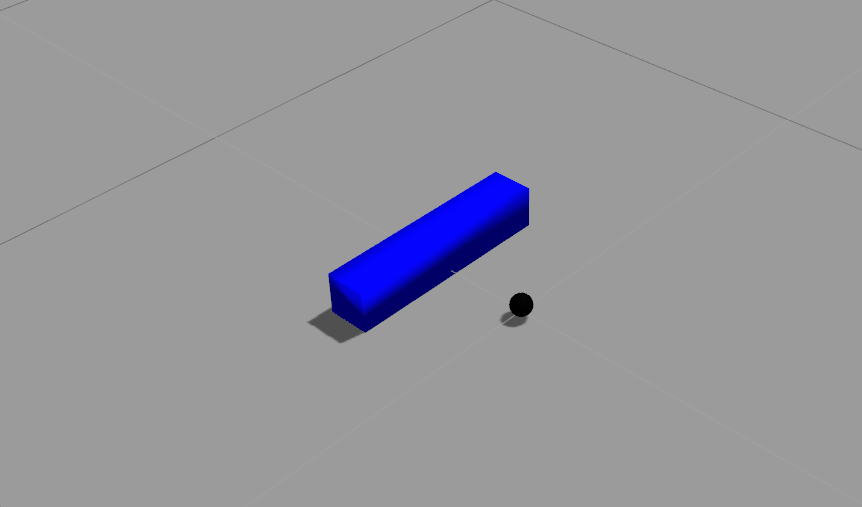
\includegraphics[width=5cm]{images/gazeboWorld.png} %TODO make image
	\caption{Overview of the used world and objects. The sphere represents the 
	robot's actuator and the rectangular block represents the primary object.}
	\label{fig:gazeboWOrld}
\end{figure}


\subsection{Communication}
In order to communicate with the simulation, a plug-in was written, that publishes the properties of all objects using google protobuf \cite{protobuf}. These messages are received and unpacked by a custom python interface that handles the communication with the simulation from the model's side. The plug-in also interprets the commands coming from the interface. A list of all implemented commands can be found in table \ref{tab:commands}

\begin{table}
	\centering
\begin{tabular}{|c|c|}
	\hline \textbf{Command} & \textbf{Meaning} \\ 
	\hline Move Command & Sets the velocity for the actuator \\ 
	\hline Pause & Pauses the simulation \\
	\hline Unpause & Continues the simulation \\
	\hline Reset & Resets the world to starting configuration \\
	\hline Set Pose & Places a specified object at a certain position \\
	\hline
\end{tabular} 
\caption{Overview of all the commands implemented in the model.}
\label{tab:commands}
\end{table}



\section{Technologies\label{sec:usedTec}}

This section briefly describes the technologies that were used or adapted to 
build the model.

\subsection{Case based Reasoning\label{sec:CBR}}
%TODO make properly!
Case based reasoning (CBR) is a delayed...
In CBR a case, in this case an episode, consists of an initial state, an 
optional action or event, and the resulting state after the action or event has 
taken place. In CBR these cases are simply stored. Whenever a new situation is 
to be handled, the case whose initial state and action are most similar to the 
current situation and available actions is retrieved and the resulting state is 
used to make a prediction about the effect of each action. Inversely, by 
searching for the resulting states, one can also decide what kind of actions 
should be taken in order to achieve a certain desired state. 


\subsection{Instantaneous Topological Map \label{sec:ITM}}
Talk about :
\begin{itemize}
	\item Similarity/difference to GNG
	\item Extension to provide output
	\item How is it trained
	\item How does it make predictions
	\item How does it return an action/preconditions
\end{itemize}

\subsection{Decision Tree}

\subsection{Learning Vector Quantization}
  \chapter{Evaluation\label{chap:evaluation}}

This chapter describes the different evaluation scenarios that were used to test the trained model 
as well as present the achieved results in each of these scenarios. The presented tests were 
designed to measure the forwards models as well as the inverse models performances. The first 
scenario, called the \enquote{Push Task Simulation}, tests the forward models of the different 
concept, while the second test scenario, the \enquote{Move to target}, tests the inverse models.

\section{Push Task Simulation}

This task is designed to test the accuracy of the forward models by decoupling them from the open 
world during successive predictions. 

\subsection{Scenario description}

In this test, the actuator uses a constant action in order to first move towards the block and then push it.
The actuator starts at different starting positions on a line parallel to the block so that the distance along
the action axis always starts at 25cm between the two centers. The block is orientated so that it's main axis
is perpendicular to the action axis.

The model is first trained using the open loop. This means that the model receives all information about the
world at each timestep before making the prediction for the next timestep. This training is done for a set amount
of \enquote{runs}. A run starts when the actuator performs the first action from the starting position and ends after a fixed 
number of iterations or if the actuator travels a predefined distance.
An example starting and end configuration can be seen in figure \ref{fig:pushTaskSim}. 

All starting positions except the first three are chosen randomly, but using the
same seed for all models and configurations. %TODO does not work, not even with the same model just with state3 vs state4... investigate!
The first three are chosen so that the actuator touches the object on the outer left, the outer right side
and directly at the center. This has been done to ensure that the models have seen all general interactions for when they are evaluated with only 3
runs. The random start positions are chosen in such a range, that the actuator can also pass the object without touching it, by sampling starting positions
between -0.35 and 0.35. Another seed is set after the training is done, so that all models are tested on the same starting positions, regardless of
the number of training examples.

The number of iterations used here is 150 when using
the model at 100Hz. During these iterations the actuator moves approximately 75cm. The maximal distance is set to 1m when using the
model with 10Hz. The actual action is the same for both frequencies and is that to 0.5m/s upwards towards the block from the starting
position. 

\begin{figure}
%TODO make figure !

\caption{TODO Push Task Simulation. The left side shows one exemplary start configuration, while on the right the corresponding end configuration can be seen.
The darker objects (dark blue and black) represent the actual block and actuator, while the transparent objects symbolize the predicted objects.}
\label{fig:pushTaskSim}
\end{figure}


\subsection{Evaluation criteria}

This task tries to evaluate the precision of the different models. In order to measure this precision, the predicted actuator position
is compared with the actual actuator position. Since at least the block can also rotate around the third axis, the orientation needs to be
considered as well when measuring the prediction performance. Since it is hard to find a metric that adequately combines point differences with
angular differences, the orientation is indirectly measured. In addition to the center position of each object, two key points are defined that
are located at the edges of the block as can be seen in figure \ref{fig:refPoints}. This way the euclidean distance can be used to measure the
prediction accuracy of both the object's position as well as their orientation. The three distances are then averaged to compute the final difference
score s:

\begin{math}
s = \frac{1}{3} \sum\limits_{i=1}^{3}||p^{pred}_i-p^{actual}_i||
\end{math}

where $p^{pred}_i, pred^{actual}_i$ represents the i's predicted and actual reference point, including the center, respectively.

These scores are computed at each timestep and accumulated. Furthermore, the final difference, at the last timestep of each run is recorded separately.
The results show the averaged results for the final difference, the accumulated differences and the mean difference over 20 test runs. The mean difference
is computed by dividing the accumulated difference by the number of predictions, the model made in each run, which is equal to the number of iterations-1. For the
first iteration, there has not been a prediction that can be compared yet.

\begin{figure}
%TODO make image

\caption{TODO Image of the reference points of the block object. The two selected edges, along with the center of the block, make up the three points that are used
to compare the predicted position with the actual position.}
\label{fig:refPoints}
\end{figure}

\subsection{Results}
%TODO 
[TODOSome first results of the interaction model. Not perfectly tuned yet, as the DT often selects strange things]

\begin{table}
\begin{tabular}{|c|c|c|c|}
\hline Model configuration & Actuator final dif & Actuator cumDif & Actuator mean dif \\ 
\hline Pairwise AC DT 3 Train & 0.001 & 0.095 & 0.001  \\ 
\hline Pairwise AC DT 10 Train & 0.053 & 3.929 & 0.026  \\ 
\hline Gate HG HA 3 Train & 0.001 & 0.128 & 0.001 \\
\hline Gate HG HA 10 Train ITM $\eta$ 0.0 & 0.001 & 0.127 & 0.001 \\ 
\hline Gate HG HA 10 Train ITM $\eta$ 0.1 & 0.001 & 0.122 & 0.001 \\
\hline Gate HG HA 10 Train ITM $\eta$ 0.2 & 0.001 & 0.122 & 0.001 \\ 
\hline Gate HG HA 10 Train NoAV & 0.001 & 0.135 & 0.001 \\ 
\hline Gate HG HA 10 Train NoDyns & 0.001 & 0.130 & 0.001 \\ 
\hline 
\end{tabular} 
\caption{Test1}
\end{table}

\begin{table}
\begin{tabular}{|c|c|c|c|}
\hline Model configuration & Block final dif & Block cumDif & Block mean dif \\ 
\hline Pairwise AC DT 3 Train & 0.209 & 14.051 & 0.094  \\ 
\hline Pairwise AC DT 10 Train & 0.142 & 10.841 & 0.073  \\
\hline Gate HG HA 3 Train & 0.048 & 3.061 & 0.021 \\ 
\hline Gate HG HA 10 Train ITM $\eta$ 0.0 & 0.052 & 3.189 & 0.021 \\ 
\hline Gate HG HA 10 Train ITM $\eta$ 0.1 & 0.046 & 2.968 & 0.020 \\ 
\hline Gate HG HA 10 Train ITM $\eta$ 0.2 & 0.061 & 3.538 & 0.024 \\ 
\hline Gate HG HA 10 Train NoAV & 0.050 & 2.859 & 0.019 \\ 
\hline Gate HG HA 10 Train NoDyns & 0.068 & 4.670 & 0.031 \\ 
\hline 
\end{tabular} 
\caption{Test2}
\end{table}

%TODO Also test only interaction prediction performance, by removing all the instances where only the gripper moved!



\section{Move to target}

\subsection{Scenario description}

\subsection{Evaluation criteria}

\subsection{Results}
  \chapter{Conclusion\label{chap:conclusion}}


\begin{itemize}
\item Discuss single timestep decision
\item Discuss results/different concepts/models
\item Reference state of the art and compare if possible
\item discuss limitations/possible improvements (of concept/implementation separately)
\end{itemize}
  %\chapter{Die Vorlage}
\label{vorlage}
  
  In diesem Kapitel wird die Vorlage näher beschrieben.
  
  \section{Das Hauptdokument}
  \label{hauptdokument}

  Das Hauptdokument ist in der Datei »documentation.tex« zu finden. Diese Datei skizziert den Aufbau des Gesamtdokuments, was bedeutet, daß dieses Dokument zum kompilieren verwandt werden muß.
    
    \subsection{Aufbau des Dokuments}
    
    Das Dokument ist bereits so aufgebaut, wie es für unsere Zwecke genügen sollte. Am Anfang binden wir eine sogenannte »Header«-Datei ein, die sämtliche Information über den Textsatz enthält. Abschnitt \ref{aufbauheader} geht genauer auf diese Datei ein.
    
    \designbox{Einbindung der »Header«-Datei}{
      \texttt{ $\backslash$input\{contents/0\_header\} }
    }
    
    Danach beginnt der Befehl für den Anfang des Dokuments. Ein TeX-Dokument muß immer mit dem Befehl \texttt{$\backslash$begin\{document\}} begonnen werden.
    
    Die Einleitung des Dokuments ist folgendermaßen aufgebaut.
    
    \begin{itemize}
      \item Titelseite
      \item Abstract
      \item Inhaltsverzeichnis
      \item Bildverzeichnis
      \item Tabellenverzeichnis
    \end{itemize}
    
    Hiernach wechseln wir die Nummerierung auf arabisch und beginnen mit dem Hauptteil der Arbeit. Jetzt werden alle Kapitel eingebunden. Da alle Kapitel in separaten Dateien abgelegt sind, müssen diese natürlich in der gewünschten Reihenfolge eingefügt werden.
    
    Direkt danach folgt der Anhang, der auf jeden Fall folgende Dinge enthält
    
    \begin{itemize}
      \item Abkürzungsverzeichnis
      \item Glossar
      \item Eidesstattliche Erklärung
      \item Literaturverzeichnis
      \item Anhang mit Material/Fragebögen usw.
    \end{itemize}
    
    
    \subsection{Stil des Literaturverzeichnisses}
    
    Als Mitglieder der TechFak verwenden wir den Zitatstil »alphadin«. Dies ist Standard für naturwissenschaftliche Texte in Deutschland und unterscheidet sich stark von »apastyle«, der bevorzugt in psychologischen Arbeiten verwendet wird.


  \section{Ein Kapitel}

  Wie eine Kapiteldatei benannt wird ist nicht sonderlich wichtig. Es ist entscheidend, daß der Dateiname ohne seine Endung korrekt in die Hauptdatei (vgl. Abschnitt \ref{hauptdokument}) eingebunden wird.

    \subsection{Aufbau}
    
    Jedes Kapitel beginnt mit dem Befehl \texttt{$\backslash$chapter\{Kapitelname\}}. Der Befehl \texttt{$\backslash$label\{kapitelname\}} definiert einen Verweisnamen, damit wir später im Dokument darauf zugreifen können. Wenn ich nun folgendes im Dokument schreibe, dann nehme ich bezug auf dieses "Label":

    \designbox{Referenz auf ein Label}{
      … wie wir in Kapitel $\backslash$ref\{kapitelname\} sehen …
    }

    TeX weiß nun, daß es die Kapitelnummer von exakt diesem Kapitel einfügen muß. D.h. die Kapitelnummer ändert sich immer auf exakt das richtige egal, ob man vorher noch 5 Kapitel einschiebt oder was auch immer.
    
    \subsection{Hierarchieebenen}

    Die Hierarchieebenen des Dokuments sind folgendermaßen:
    
    \begin{itemize}
      \item $\backslash$chapter
      \item $\backslash$section 
      \item $\backslash$subsection 
      \item $\backslash$subsubsection 
      \item $\backslash$paragraph
      \item $\backslash$subparagraph
    \end{itemize}

    Labels kann man auch jedem dieser Elemente verpassen, so daß man sich auch direkt darauf beziehen kann.   


  \section{Der Kopf bzw. Header}
  \label{aufbauheader}

  Die Datei »0\_header.tex« ist das Herzstück das Dokuments. Hier wird das komplette Aussehen des Dokuments bestimmt. D.h. man kann diese Datei austauschen und das ganze sieht komplett anders aus. Der Vorteil: es ist rein gar nichts am geschriebenen Text in den Kapiteln zu ändern!
  
  Die Datei ist gut kommentiert und eigentlich selbsterklärend. Es ist wichtig, die Einstellungen für das PDF zu ändern, so daß sichergestellt ist, daß die Stichwörter, Autoren usw. zum Dokument passen.


  \section{Literatur und Referenzen}

  In der Datei »D\_referenzen.bib« befindet sich die Literatur. Sie ist dort im BibTeX-Standard abgelegt. Ein Beispieleintrag sähe nun folgendermaßen aus:
  
  \designbox{Beispiel für BibTex}{
    \fontspec[Color=101010, Scale=0.8]{Courier}
    @book\{badura99,
    
      ~~title=\{\{Psychologie in der Praxis\}\},
      
      ~~author=\{Badura, B. and Ritter, W.\},
      
      ~~year=\{1999\},
      
      ~~publisher=\{Bohn-Verlag, Berlin\}
      
    \}
  }

  Diese Einträge kann man entweder selbst erstellen oder einfacher: man benützt dafür GoogleSchoolar oder CiteSeerX. Man sollte allerdings unvollständige Einträge selbst ergänzen, um so ein ordentliches Literaturverzeichnis, welches wissenschaftlichen Standards entspricht, zu erhalten. 
  
  Das einzige, was per Hand anpaßt wird, ist der Kurzname (im obigen Beispiel »badura99«). Dieser Kurzname wird benötigt, wenn man sich im Dokument darauf bezieht. Im Text zitiere ich nun folgendermaßen:

  \designbox{Zitate einfügen}{
  Nach $\backslash$cite\{badura99\} ergab das ganze ein tolles Ergebnis.
  }

  Im Literaturverzeichnis tauchen nur Sachen auf, die man wirklich zitiert hat (es gibt natürlich auch Möglichkeiten trotzdem Dinge aufzunehmen, die man nicht zitiert). Ebenfalls sieht man im Dokument, welche Verweise man im Literaturverzeichnis vergessen hat! Hier erscheinen hinterher Einträge à la [?] auf. Diese sollte man vor Abgabe der Arbeit dringend überprüfen und entsprechend korrigieren.


  \section{Test}
  \label{test}
  
    \subsection*{Sektion ohne Eintrag}
    
    Ich bin eine Sektion, die nicht im Inhaltsverzeichnis auftaucht. Dies erreiche ich durch einen \texttt{*}.
    
    \subsection*{Sektion, die zweite}
    
    \begin{figure}[h!]
      \centering
      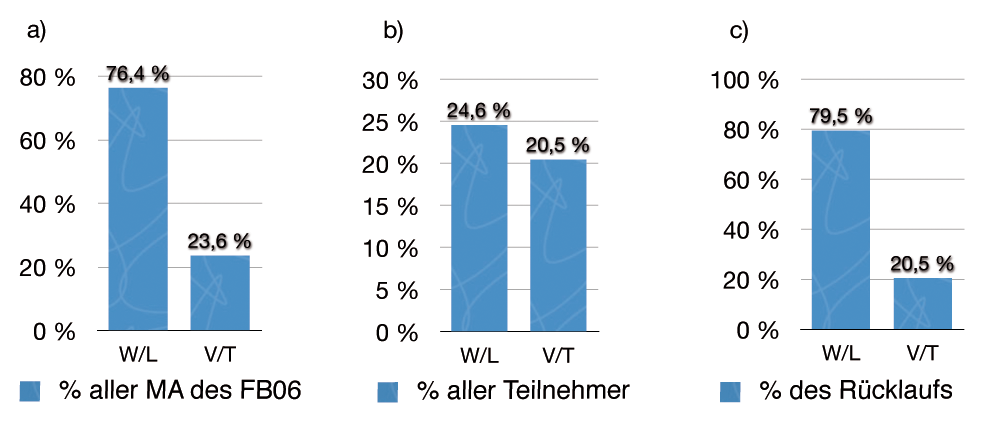
\includegraphics[width=11cm]{bilder/bild1.png} 
      \caption{Ich bin die Beschreibung und bin wichtig}
      \label{bild1}
    \end{figure}
    
    Abbildung \ref{bild1} zeigt die prozentuale Verteilung der Dienstbereiche im Fachbereich. 76,4\% der insgesamt 165 Mitarbeiter arbeiten in den Dienstbereichen Wissenschaft und Lehre (W/L, n = 126), 23,6\% in den Bereichen Verwaltung und Technik (V/T, n~=~39). 

    \subsection*{Tabellen}
    
    Wie in Tabelle \ref{tabelleBeteiligungsverhaeltnis} dargestellt ist, lag die Beteiligung der weiblichen Mitarbeiter mit knapp 53\% leicht über der der männlichen Mitarbeiter mit gut 47\%.
        
    \begin{table}[h]
      \centering
      \caption{\label{tabelleBeteiligungsverhaeltnis} Beteiligungsverhältnis Männer/Frauen}
      \begin{tabular}{|l|c|c|c|c|} \hline
        \multicolumn{2}{|c|}{} & \multicolumn{2}{c|}{\textbf{Geschlecht}} & \multirow{2}{*}{\textbf{Gesamt}} \\  \cline {3-4}
        \multicolumn{2}{|c|}{} & weiblich & männlich & \\ \hline
        \textbf{Dienst-} & Wissenschaft/Lehre & 14 & 16 & 30 \\ \cline{2-5}
        \textbf{bereich} & Verwaltung/Technik & 6 & 2 & 8 \\ \hline
        \multicolumn{2}{|l|}{Gesamt} & 20 (53\%) & 18 (47\%) & 38 (100\%) \\ \hline
     \end{tabular}
   \end{table}
   
   Alle Tabellen sind natürlich als TeX in das Dokument eingefügt und gehen damit ins Tabellenverzeichnis ein; sie werden nicht fälschlicherweise als Bild aufgeführt. Einen guten Editor für TeX sollte man allerdings dafür besitzen. Ein für alle Betriebssysteme verfügbarer Editor ist z.B. Kile. Eine andere Möglichkeit sind spezielle Tabellenkonverter. Dazu befragt man am besten das Repository seines Betriebsystems.

    
    \subsection*{Ein anderes Bild}
    
    Mit etwa 34\% ist die Gruppe der 30- bis 39jährigen Mitarbeiter in dieser Stichprobe am größten. Darauf folgen die 20- bis 29jährigen Mitarbeiter mit gut 26\% (s. Abb. \ref{bild2}; n~=~38).
    
    \begin{figure}[ht]
      \centering
      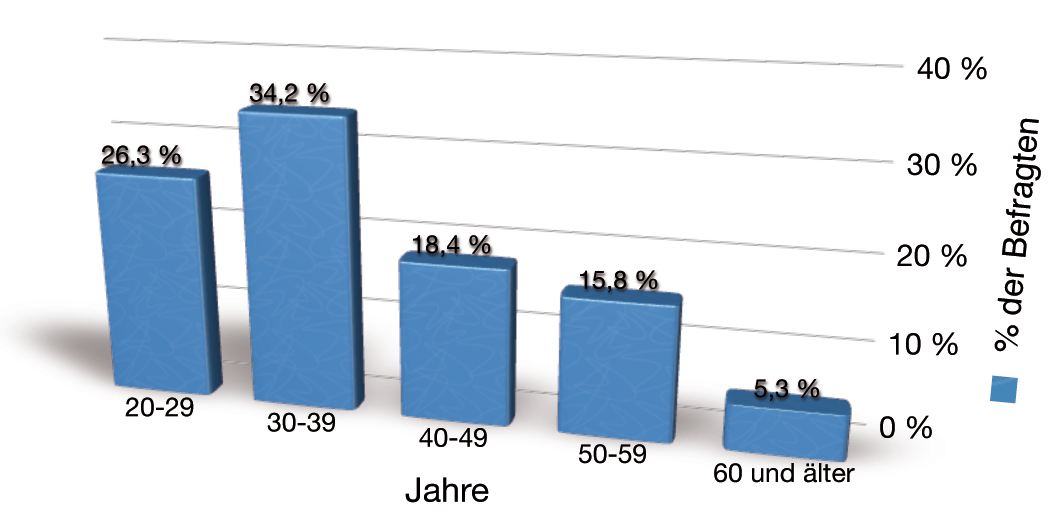
\includegraphics[width=9cm]{bilder/bild2.png} 
      \caption{Erklärung findet man hier}
      \label{bild2}
    \end{figure}
    
    \subsubsection*{Tätigkeitsdauer}
    
    Mehr als 50\% der Befragten sind seit einem Zeitraum von bis zu fünf Jahren an der Universität beschäftigt. Die nächstgrößere Gruppe arbeitet seit sechs bis zehn Jahren an der Universität (s. Abb. \ref{bild3}; n~=~39). 
    
    \begin{figure}[h]
      \centering
      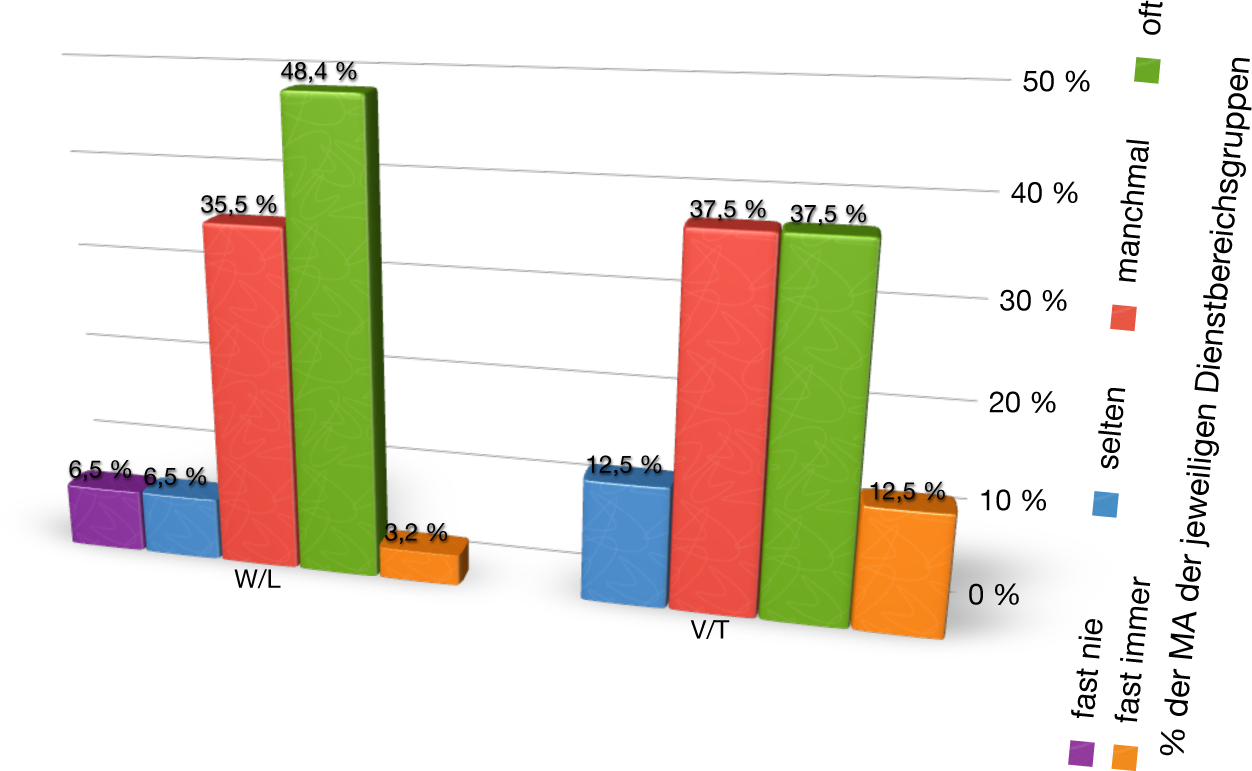
\includegraphics[width=12cm]{bilder/bild3.png} 
      \caption{Beschreibung}
      \label{bild3}
    \end{figure}

  \section{Schlußwort}
  \label{schluszwort}
  
  Die Darstellung der Graphiken und Tabellen im gesamten Abschnitt \ref{test} beziehen sich auf alle 429 Teilnehmer der Umfrage.

  %\chapter{Motivation}



  %\chapter{Fazit und Ausblick}

In dieser Arbeit haben wir gezeigt, daß es möglich ist auch ohne WYSIWYG\footnote{What you see is what you get}-Editor ein Dokument erstellen können.

Wir werden mit folgendem noch sicherstellen, daß wir auch alle Zitate in unserem Literaturverzeichnis haben (vgl. \cite{abel92, badura09, burrows05}).
  
  \bibliographystyle{alphadin}
  \bibliography{contents/D_references}
  % Anhang
  \appendix
  %\chapter{Akronyme und Abkürzungen}

\begin{description}
  \item[GCC] GNU Compiler Collection
  \item[UTF-8] 8-bit Unicode Transformation Format
  \item[XML] Extensible Markup Language
\end{description}


  %\chapter{Glossar}

\begin{description}
  \item[POSIX] beschreibt etwas ganz interessantes.
  \item[Standard input/output] Eine Beschreibung für das Element.
\end{description}

  % Eidesstattliche Erklärung

% Dieser Text wurde aus dem Landesgesetz übernommen und ist nicht zu ändern!

\chapter{Eidesstattliche Erklärung}

  Ich versichere hiermit, daß ich die vorliegende Arbeit selbständig verfaßt und keine anderen als die im Literaturverzeichnis angegebenen Quellen benutzt haben.

  Alle Stellen, die wörtlich oder sinngemäß aus veröffentlichten oder noch nicht veröffentlichten Quellen entnommen sind, sind als solche kenntlich gemacht.

  Die Zeichnungen oder Abbildungen in dieser Arbeit sind von mir selbst erstellt worden oder mit einem entsprechenden Quellennachweis versehen.

  Die Arbeit ist in gleicher oder ähnlicher Form noch bei keiner anderen Prüfungsbehörde eingereicht worden.

  Bielefeld, den XX. Monat 20XX

  \vspace*{1.5\baselineskip}
  
  \begin{table}[ht!]
    \begin{center}
      \begin{tabular}{p{120pt}p{50pt}p{120pt}}
        ~ & ~ & ~\\ \cline{3-3}
        ~ & ~ & Nachname, Vorname\\
      \end{tabular}
    \end{center}
  \end{table}




  %\chapter{Additional Information}

\section{Circling action \label{sec:circling}}

The circling action was designed to make do with the features available where possible.
For the interaction model the distance between the actuator and block needed to be computed as well. The distance is required since the explicit use of object shape information outside of the distance computation was not desired. 
The process is described in algorithm \ref{alg:circling}:

\begin{algorithm}
\begin{algorithmic}[1]
\Require{Distance $dist$ between actuator and object}
\Require{Local direction $\vec{d}_{local}$ from actuator to object}
\Require{Global direction $\vec{d}_{global}$ from actuator to object}
\Require{Local direction $\vec{t}$ from target to object}
\Ensure{Velocity vector $\vec{v}$ that moves the actuator around the object towards the target.}
\Statex
\If{$dist < 0.04$} 
	\Let{$\vec{v}$}{$-{norm} \cdot \vec{d}_{global}$} 
\ElsIf{$dist$ > 0.06} 
	\Let{$\vec{v}$}{${norm} \cdot \vec{d}_{global}$} 
\Else 
	\Let{$\vec{v}$}{computeTangent( $\vec{d}_{global}$, $\vec{d}_{local}$, $\vec{t}$)}  
\EndIf
\State \Return{$\vec{v}$}
\Statex
\Function {computeTangent}{$\vec{d}_{global}$, $\vec{d}_{local}$, $\vec{t}$}
	\Let{$\vec{tan}$}{$[-\vec{d}_{global}[1], \vec{d}_{global}[0]]$}
	\State \Return{$\vec{tan}$}
\EndFunction
\end{algorithmic}
\caption{Pseudocode for computing a suitable circling action.}
\label{alg:circling}
\end{algorithm}


Using the distance, the actuator can stay within a save distance of \m{0.04} to \m{0.06} of the object. Outside this area, the actuator moves straight towards or away from the center of the object. This ensures, that the actuator does not collide with the object while circling.
Inside this area, the actuator uses one of the two tangents to the global direction from the actuator to the object. Which tangent to use is determined by the angles of the vectors between actuator-object and target-object with respect to the local x axis of the objects coordinate system. 
The direction, that reduces the difference the most is chosen.

\section{Protobuf messages \label{sec:protobufMessages}}

%
%  Hier steht Text.
%
%  \section{Quelltexte}
%
%  Hier steht auch Text.
%
%    \subsection{Algorithmus 1}
%
%    Hier kommt ein Quelltext.
%
%    \begin{lstlisting}[caption=Standard-Quelltext, label=simple_main]
%      int main (int args, char** argv)
%      {
%        return 0;
%      }
%    \end{lstlisting}
%
%
%    \subsection{Fragebogen}
%
%    Hier ist ein Muster eines Fragebogens, den ich verwendet habe.

\end{document}
